\Exercise{Ein Formular gestalten}
%
\par Verwenden Sie als Grundlage die Lösung von Aufgabe 9 auf dem zweiten Übungsblatt. Sie können auch meinen Lösungvorschlag herunterladen und mit diesem weiterarbeiten. Ändern Sie das Formular durch Einsatz von CSS so ab, dass es am Ende folgendermaßen aussieht:
%
\begin{figure}[!h]
\centering
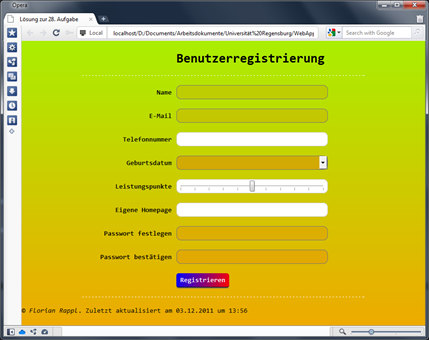
\includegraphics[width=0.5\textwidth]{Figures/form.png}
\caption{Ansicht des Formulars mit dem eingefügten CSS}
\label{fig:form}
\end{figure}
%
\par Hierbei sollten Sie v.a. folgende Einstellungen beachten:
%
\begin{itemize}
\item Als Schriftart verwenden Sie ``Consolas'', ``Andale Mono'', ``Lucida Console'', ``Courier New'', monospace mit einer Größe von \qty{14}{px}.
\item Der Hintergrund ist ein Farbverlauf (unten nach oben) von \hcolor{AE0} auf \hcolor{EA0}.
\item Das Formular hat eine Breite von \qty{600}{px} und ist immer zentriert (aber nicht absolut!) ausgerichtet.
\item Ober- und Unterhalb des Formulars ist eine gestrichelte (weiße) Linie.
\item Die Labels des Formulars sollen eine Breite von \qty{200}{px} besitzen und rechtsbündig ausgerichtet sein.
\item Die Eingabeelemente besitzen eine Breite von \qty{300}{px} mit \qty{10}{px} inneren Abstand. Die Ecken sind abgerundet mit einem Radius von \qty{10}{px}.
\item Der Button soll ein völlig eigenes Design besitzen mit einer Höhe von \qty{30}{px} und einem Farbverlauf von \hcolor{F00} (links oben) nach \hcolor{00F} (rechts unten). Er hat einen dezenten Schatten und \qty{5}{px} runde Ecken.
\item Die notwendigen Textfelder sind speziell hervorgehoben: Der Rahmen ist dunkler und als Hintergrund wurde \jvar{rgb(255, 20, 20)} mit einem Alpha-Wert von \qty{10}{\%} verwendet!
\end{itemize}